\documentclass[border=10pt]{standalone}
\usepackage[T1]{fontenc}
\usepackage{tikz}
\usetikzlibrary{positioning, arrows.meta, calc, fit}

\definecolor{accent}{HTML}{1E3A8A}
\definecolor{boxfill}{HTML}{F1F5F9}
\definecolor{boxstroke}{HTML}{475569}

\begin{document}
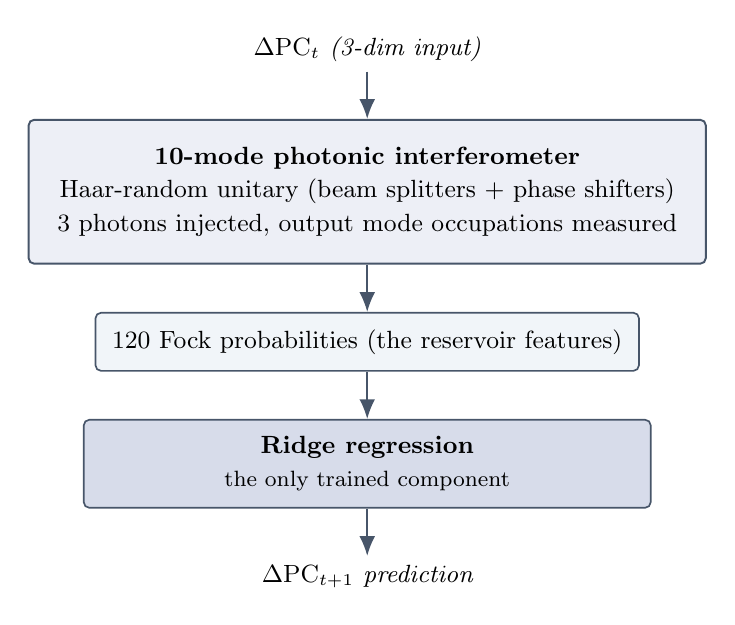
\begin{tikzpicture}[
  every node/.style={font=\small},
  >={Latex[length=2.5mm, width=2mm]},
  box/.style={
    draw=boxstroke, line width=0.6pt, fill=boxfill,
    rounded corners=2pt, inner sep=6pt,
    align=center
  },
  bigbox/.style={
    draw=boxstroke, line width=0.7pt, fill=accent!8,
    rounded corners=2pt, inner sep=10pt,
    minimum width=86mm, align=center
  },
  arrow/.style={->, line width=0.6pt, draw=boxstroke}
]

\node[font=\small\itshape] (input) {$\Delta\mathrm{PC}_t$ (3-dim input)};

\node[bigbox, below=6mm of input] (interfero) {%
  \textbf{10-mode photonic interferometer} \\[1pt]
  Haar-random unitary (beam splitters + phase shifters) \\[1pt]
  3 photons injected, output mode occupations measured};

\node[box, below=6mm of interfero] (fock) {120 Fock probabilities (the reservoir features)};

\node[box, below=6mm of fock, fill=accent!18, minimum width=72mm] (ridge) {%
  \textbf{Ridge regression} \\[1pt]
  \footnotesize the only trained component};

\node[font=\small\itshape, below=6mm of ridge] (output) {$\Delta\mathrm{PC}_{t+1}$ prediction};

\draw[arrow] (input) -- (interfero);
\draw[arrow] (interfero) -- (fock);
\draw[arrow] (fock) -- (ridge);
\draw[arrow] (ridge) -- (output);

\end{tikzpicture}
\end{document}
